\section{Repairing Strategy: Exception Type}
\label{sec:strgEx}

%marker
%textcolor{red}{\textbf{Please review this section}}\newline

\begin{figure}[t]
\lstset{language=Java, caption=Java code which may throws runtime exceptions,
label=example1}
\begin{lstlisting}[countblanklines=false]
public class TestClass {
    private int[] arr1;
    private int[] arr2;
    private int[] arr3;

    public TestClass(int[] arr1, int[] arr2, int[] arr3) {
	this.arr1 = arr1;
	this.arr2 = arr2;
	this.arr3 = arr3;
    }
    public int[] fun(int a, int b, int c, int d) {
	int temp0 = a + b;
	int temp1 = c * d;
	int temp2 = temp0 - temp1;
	//array index out of bound, negative index
	int temp3 = this.arr1[temp0];
	//array index out of bound, negative index
	int temp4 = this.arr2[temp1];
	//array index out of bound, negative index
	int temp5 = this.arr3[temp3];
	int temp6 = temp4 + temp5;
	int temp7 = temp6 - temp3;
	//array index out of bound, negative index, divide by zero
	this.arr1[temp6] = temp7/(d-a);
	//array index out of bound, negative index, divide by zero
	this.arr2[temp7] = temp7/temp4;
	if(arr2[temp1] ! = arr3[temp7]) return arr1;
	else return null;
    }
}
public class MainClass {
    public void main(String[] a) {
	int[] arr1 = {1,2,3,4};
	int[] arr2 = {1,2,3,4};
	int[] arr3 = {1,2,3,4};
	TestClass TC = new TestClass(arr1, arr2, arr3);
	int[] res = TC.fun(2,4,3,4);
	//Null pointer exception
	System.out.print("Result : "+res[2]);
    }    
}
\end{lstlisting}
\end{figure}

In the Example~\ref{example1}, we have given a piece of \java\ code which shows
multiple lines can throw several runtime exceptions.
In this example we consider three very common runtime exceptions:
NullPointerException, ArrayIndexOutOfBoundExcepltion, NegetiveIndexException,
ArithmeticException (i.e. divide-by-zero). In rest of this section, this
particular example will be used to demonstrate the repairing strategy.

\subsection{Symbolic Analysis}
\label{subsec:symb}

\begin{figure}[t]
\centering
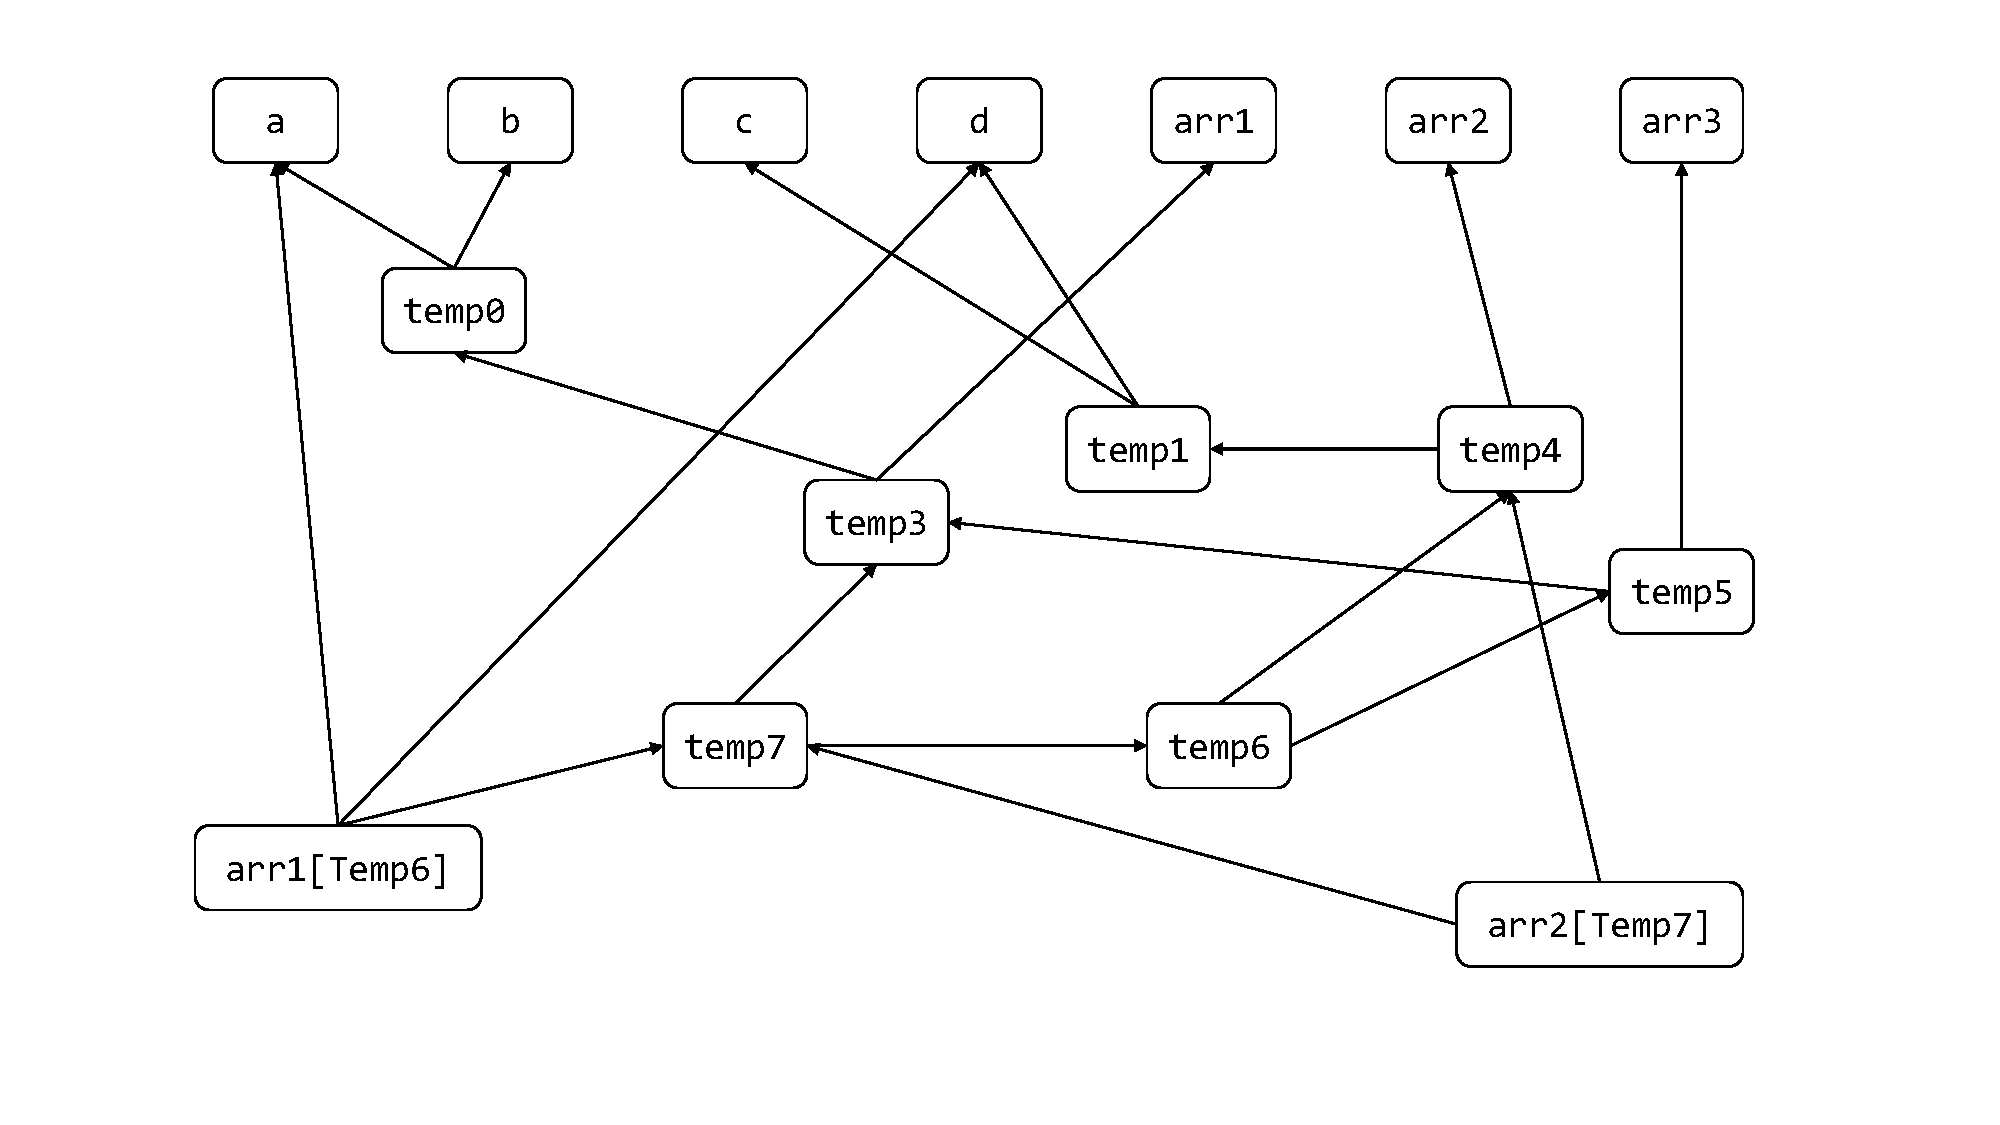
\includegraphics[width=3.3in]{images/depG.pdf}
\caption{Data dependency graph of the variables in Example\ref{example1}}
\label{fig:datadep}
\end{figure}

We have done several  static analysis a priori  over the Java source code to
discover :
\begin{mylist}
\item Critical section of the code which are not eligible for patching. Eg.
banking or any financial transaction which should be crashed in case of
exception as suboptimal solution due to patching will led it to inconsistent
state.
\item Symbolic analysis of the program to discover potential points of failure
and mark them.
\item Build data dependency graph which will be used to generate appropriate
code slice to be used as patch.
In Figure~\ref{fig:datadep}, the data dependency graph of the example
code~\ref{example1} is presented.
\item The symbolic analysis will also reveal which kind of exception is likely
to happened at the time of execution.
This information is necessary at the time of instrumenting the patch as it will
determine the catch block.
	
\end{mylist}

\subsection{Data set for Successful Program Runs}
\label{subsec:progrun}

Here we will store all the traces of successful program runs.
\begin{figure}[t]
\centering
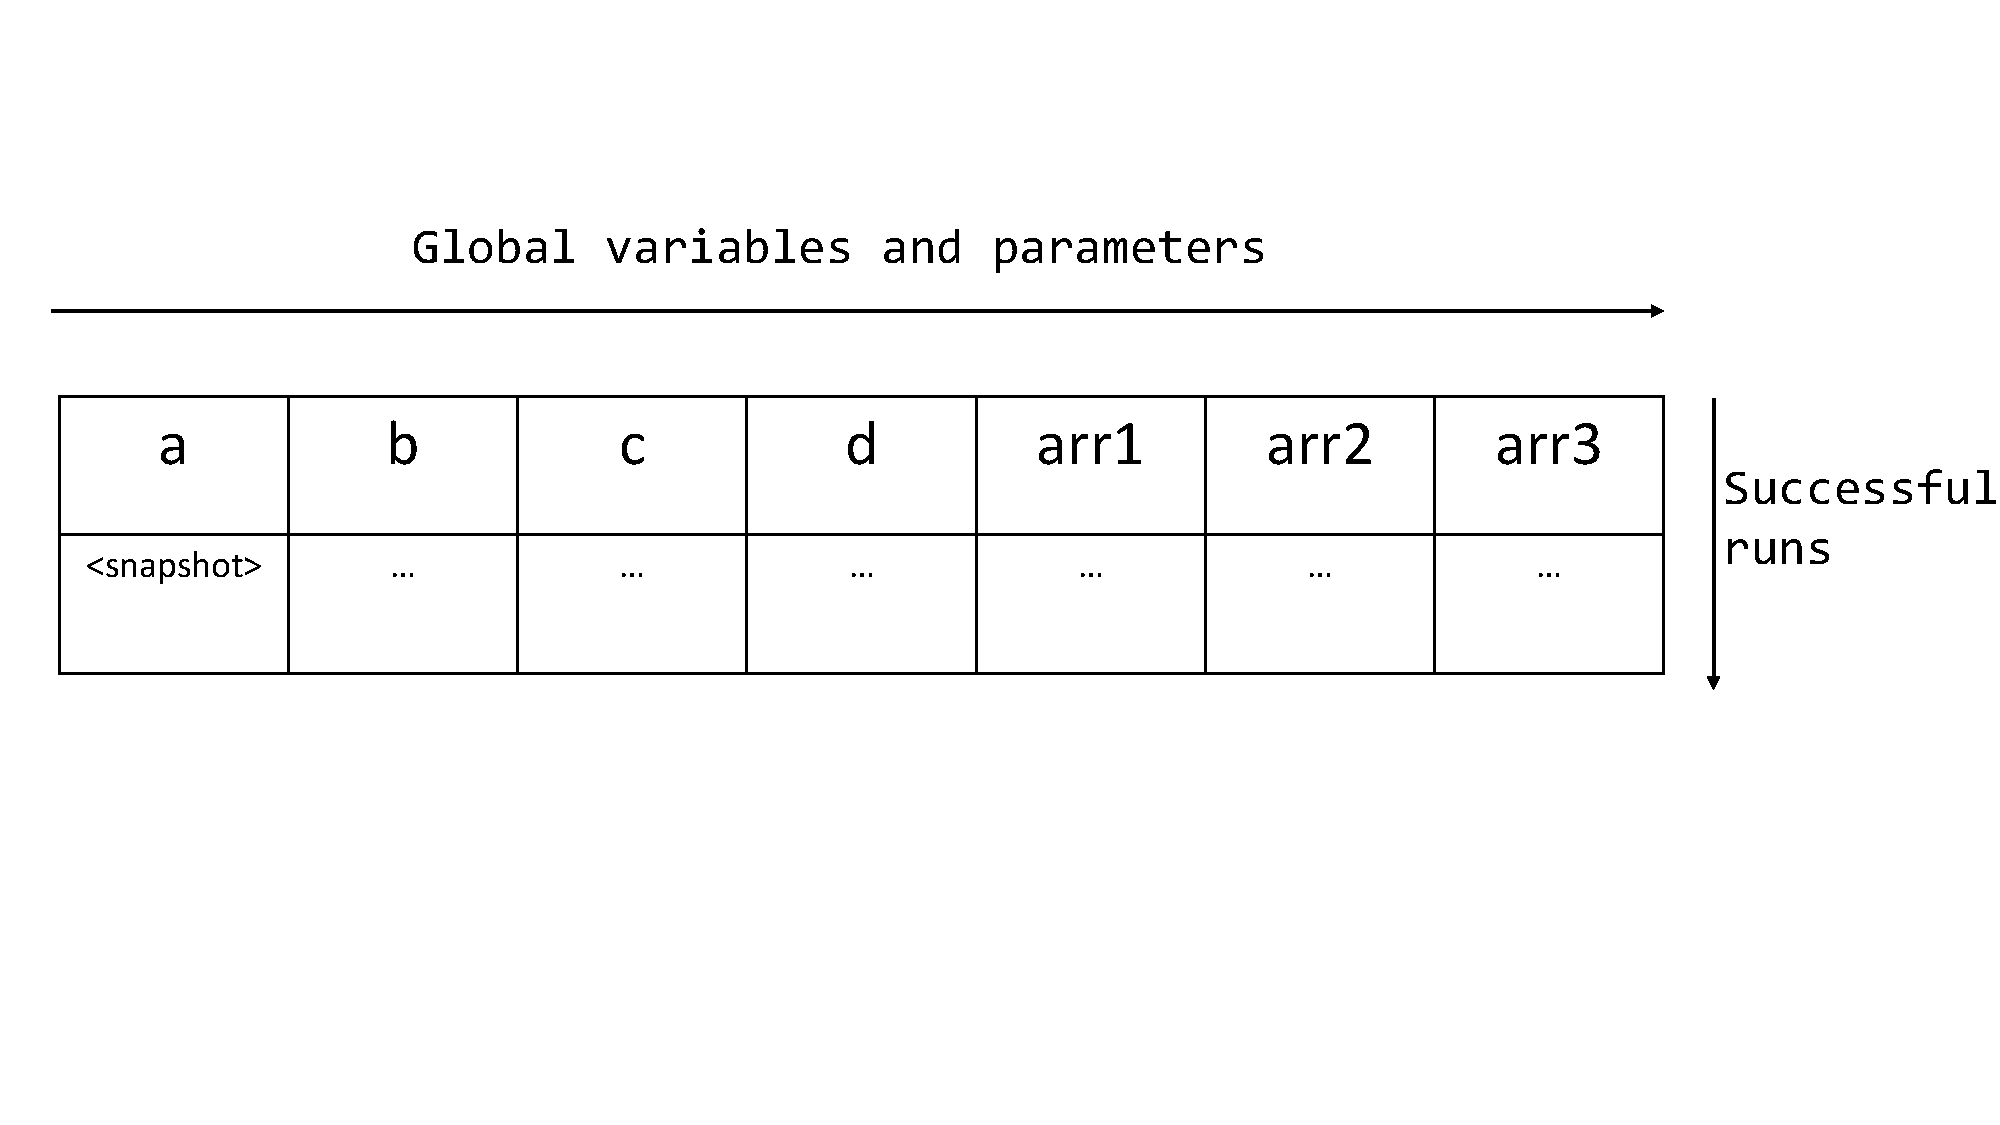
\includegraphics[width=3.0in]{images/succrun.pdf}
\caption{Indexed global variables and method arguments successful runs}
\label{fig:succrun}
\end{figure}

Figure~\ref{fig:succrun} shows such indexed traces of all the global variables
and method arguments.
We store the snapshots of these objects. We won't store local variables as they
can always be regenerated.
As it is required to capture the snapshot of all these variable, we made deep
cone of all of these objects and variables.

% begin{table}[htb]
%\begin{tabular}{|c|c|c|c|c|c|c|}
%\hline
%a & b & c & d & arr1 & arr2 & arr3 \\ \hline
%\ldots & \ldots & \ldots & \ldots &	\ldots & \ldots & \ldots\\ \hline
%\end{tabular}
%\caption{Trace of successful runs}
%	\label{tab:Trace}
%\end{table}


\subsection{Matrices}
\label{subsec:martices}

%marker
%\textcolor{red}{\textbf{Please review this section.}}\newline

\subsection{Instrumenting Patching}
\label{subsec:patchinstru}

We have used Soot framework which is a Java byte code manipulator to instrument
patch. 
The patching technique is divided into two phases

\subsubsection{Determine Exception Type} 

At the time of execution, the exception may happened due to some specific values
of some variables. We will catch the exception. Here the type of runtime
exception is $java.lang.ArrayIndexOutOfBound$. This will be used to produce the
try-catch block.
 
\subsubsection{Determine Optimal Code Slice}

The optimal code slice will be determined from the data dependency graph which
was rendered at the time of static analysis mentioned in
\S~\ref{subsec:symb}. In the Listing~\ref{patchingexample1}, the example
code snippet shows such code slice inside the catch block.
As the error occurred at the line $int\ temp5\ =\ this.arr3[temp3];$ the
statements which produces the temp3 and the statement which also involves
$temp3$ or any other variables derived from $temp3$, would be included in the
catch block for re-execution with the valued of the same from the data table of
previous successful runs.

 

\lstset{language=Java, caption=patching code slice based on exception type,
label=patchingexample1}

\begin{figure}[t]
\begin{lstlisting}[countblanklines=false]
public class TestClass {
    private int[] arr1;
    private int[] arr2;
    private int[] arr3;

    public TestClass(int[] arr1, int[] arr2, int[] arr3) {
	this.arr1 = arr1;
	this.arr2 = arr2;
	this.arr3 = arr3;
    }
    public int[] fun(int a, int b, int c, int d) {
	try {
	    int temp0 = a + b;
	    int temp1 = c * d;
	    int temp2 = temp0 - temp1;
	    int temp3 = this.arr1[temp0];
	    int temp4 = this.arr2[temp1];
	    //IndexOutOfBoundException as temp3 = 20
	    int temp5 = this.arr3[temp3];
	    int temp6 = temp4 + temp5;
	    int temp7 = temp6 - temp3;
	    this.arr1[temp6] = temp7/(d-a);
	    this.arr2[temp7] = temp7/temp4;
	} catch(IndexOutOfBoundsException indEx) {
	    int temp0 = a + b;
	    int temp1 = c * d;
	    int temp2 = temp0 - temp1;
	    int temp3 = this.arr1[temp0];
	    //Bellow line is not part of the patch as
	    //temp1 and temp3are not related to temp3
	    //for which the exception occurred.
	    //int temp4 = this.arr2[temp1];
	    int temp5 = this.arr3[temp3];
	}
	if(arr2[temp1] ! = arr3[temp7]) return arr1;
	else return null;
    }
}
public class MainClass {
    public void main(String[] a) {
	int[] arr1 = {20,21,22,23};
	int[] arr2 = {1,2,3,4};
	int[] arr3 = {10,11,12,13};
	TestClass TC = new TestClass(arr1, arr2, arr3);
	int[] res = TC.fun(2,4,3,2);
	System.out.print("Result : " + res[2]);
    }    
}
\end{lstlisting}
\end{figure}

\subsection{Variable Tracking and Monitoring}
\label{subsec:taint}
%\textcolor{red}{\textbf{I have added standard taint analysis technique here as
%an example. We can change it later}}\newline


Here we used taint analysis technique to tag variables and objects of our
interest to monitor them.
This steps are necessary as the values of the variables used during the
instrumentation may cause further runtime exceptions.
We used bit-vector which is an efficient technique to taint a object/variable.
It requires maintain a single dimension byte array where each bit correspond to
a single object/variable of our interest.
The bit values will be flipped when it is required to taint ($1$) or untaint
($1$) an object/variable.
We will only monitor these entities until all of them flushed from the program
and the entire program reached to a stable state.